\documentclass[a4,12pt]{article}

\usepackage[english]{babel}
\usepackage[utf8]{inputenc}
\usepackage[T1]{fontenc}
\usepackage[proportional]{libertine}
\usepackage[libertine]{newtxmath}

% Import the natbib package and sets a bibliography  and citation styles
\usepackage[numbers]{natbib}
\bibliographystyle{plainnat}
% \setcitestyle{numbers}

\usepackage{amsmath}
\usepackage{graphicx}
\usepackage{hyperref}
\usepackage{paralist}
\usepackage{xcolor}

%%% math
\newcommand{\betap}{\ensuremath{\beta^\prime}}
\newcommand{\data}{\ensuremath{\mathcal{D}}}
\newcommand{\expin}{\ensuremath{\lbrace\mu_i, \sigma_i\rbrace}}
\DeclareMathOperator{\Dirichlet}{Dirichlet}
\newcommand{\given}[2]{\left(#1\, \middle| #2 \, \right)}
\newcommand{\gaussian}{\ensuremath{\mathcal{N}}}
\newcommand{\genbetapr}{\ensuremath{\mathrm{GenBetaPrime}}}
\newcommand{\likelihood}{\ensuremath{\mathcal{L}}}
\newcommand{\lumi}{\ensuremath{\ell_i}}
\newcommand{\Lumi}{\ensuremath{L_i}}
\newcommand{\real}{\ensuremath{{\rm real}}}
\newcommand{\virt}{\ensuremath{{\rm virt}}}
\newcommand{\Nreal}{\ensuremath{N_\real}}
\newcommand{\Nvirt}{\ensuremath{N_\virt}}
\newcommand{\poisson}{\ensuremath{\mathrm{Poisson}}}
\newcommand{\rmdx}[1]{\mbox{d} #1 \,} % differential
\newcommand{\vecalpha}{\ensuremath{\vec{\alpha}}}
\newcommand{\vecL}{\ensuremath{\vec{L}}}
\newcommand{\vecmu}{\ensuremath{\vec{\mu}}}
\newcommand{\vecnu}{\ensuremath{\vec{\nu}}}
\newcommand{\vecth}{\ensuremath{{\vec{\theta}}}}
\newcommand{\vecu}{\ensuremath{{\vec{u}}}}


\DeclareMathOperator{\erf}{erf}
\newcommand{\mui}{\mu_i}
% \newcommand{\Ni}{N_i}
% \newcommand{\ni}{n_i}
\newcommand{\sigi}{\sigma_i^2}
\DeclareMathOperator{\sgn}{sgn}
\newcommand{\El}{E[l]}
\newcommand{\Vl}{V[l]}

%%% refs
\def \refeq#1{(\ref{eq:#1})}
\def \refsec#1{sec.~\ref{#1}}
\def \refSec#1{Sec.~\ref{#1}}
\def \refapp#1{app.~\ref{#1}}
\def \reffig#1{fig.~\ref{fig:#1}}

%%% comments
\newcommand{\todo}[1]{{\textsc{\color{red}#1}}}

%%% codes
\newcommand{\tardis}{TARDIS}

\title{Formulating the posterior for \tardis}
\author{Frederik Beaujean}

\begin{document}
\maketitle

\section{Input and Output}

\subsubsection*{What we are given}
\begin{itemize}
\item data $\data \sim \expin =$ set of input values from
  telescope for each frequency bin $i=1 \dots n_b$;
\item \tardis{} depends on the parameters $\vecth$ and
  produces $n_\real$ real photon packets that leave the supernova and
  $n_\virt$ virtual photon packets. When we bin the packets in the same
  frequency bins as \expin, the sum of luminosities in bin $i$ is
  $\lumi^\real$ and $\lumi^\virt$.
\end{itemize}
I try to be mostly consistent with standard notation in statistics and
denote random variables---eventually they will be integrated out---by
capital letters and numbers that are observed by lower case.

\subsubsection*{What we want}
The posterior distribution of $\vecth$ given the data $\data$,
$P(\vecth | \data)$, is given by  Bayes' theorem as
\begin{equation}
  \label{eq:Bayes-full}
  P\given{\vecth}{\data} = \frac{P\given{\data}{\vecth} P(\vecth)}{\int \rmdx{\vecth} P\given{\data}{\vecth} P(\vecth)} \,.
\end{equation}
Technically, we should write every propability (density) as
conditional on a specific statistical model $M$,
e.g. $P\given{\vecth}{\data, M}$.  At present, we are not interested
in comparing different models but rather in extracting the parameters
of one model. Thus we omit $M$ and can ignore the denominator (the
\emph{evidence}) in Bayes' theorem. All we need is to define the
likelihood $\likelihood(\vecth) \equiv P\given{\data}{\vecth}$ and the
prior $P(\vecth)$ in
\begin{equation}
  \label{eq:Bayes-simple}
  P\given{\vecth}{\data} \propto \likelihood(\vecth) P(\vecth) \,.
\end{equation}

% Notation: $\vecth=$ parameters of interest,

% The overall goal is to extract (or maximize) the posterior of
% $\vecth$, the parameters that describe the physics behind
% supernovae. Bayes' theorem is
% \begin{align}
%   \label{eq:post}
%   P(\vecth | \mathcal{D}) &\propto P(\mathcal{D} | \vecth) P_0(\vecth)
% \end{align}
\section{Likelihood}

\subsubsection*{Goals}
\begin{itemize}
\item take into account uncertainty due to the finite number of packets in the simulation
\item model the distribution of luminosities accurately
\end{itemize}

\subsection{Incorporating the observations}

Let \Lumi{} denote the predicted or true luminosity in bin $i$ and
$\vecL$ the ordered collection of luminosities. I assume from a
telescope, we get the probability of the data $\mathcal{D}$ given
$\vecth$ only as a function of $\vecL$ where the data are
implicit---we don't have them---and no correlation between bins is
given or assumed. The maximum-entropy distribution given only the
means and standard deviations $\expin, i=1\dots n_b$ is the normal or
Gaussian distribution, so we set
\begin{equation}
  \label{eq:like-L}
  P(\mathcal{D} | \vecL) = \prod_{i=1}^{n_b} \gaussian\given{\Lumi}{\mu_i, \sigma_i^2}.
\end{equation}

In principle, $\vecL(\vecth)$ is a deterministic function of
$\vecth$. But we are unable to calculate it as is; that's why we have
to estimate it from the \tardis{} simulation resulting in a
distribution $P\given{\vecL}{\vecth}$. To use Bayes'
theorem~\refeq{Bayes-full}, we need $P\given{\data}{\vecth}$ but we
only have $P\given{\data}{\vecL}$. The link between these three
densities is the law of total probability:
\begin{align}
  \label{eq:like-expanded}
  P\given{\data}{\vecth} &= \int \rmdx{\vecL} P\given{\vecL}{\vecth} P\given{\data}{\vecL}.
\end{align}
Note that in principle it should say $P\given{\data}{\vecL, \vecth}$
in \refeq{like-expanded} but in our case $\vecth$ doesn't appear
explicitly, so we can just plug in
$P\given{\data}{\vecL}$ from~\refeq{like-L}.

To complete the specification of the likelihood, we need to formulate
$P\given{\vecL}{\vecth}$; i.e., what we learn about the luminosities
in each bin from \tardis. A simplified account of how \tardis{} is run
follows, then I will show how to phrase this in statistical terms.

\subsection{Running \tardis}
\todo{This is still rudimentary}
\begin{compactenum}[(I)]
  \item Adjust the temperature of an inner shell to approximately match
    the total luminosity inferred from the observations
  \item Choose a total number of real packets, and a number of virtual
    packets to send out on each scattering of a real packet.
  \item Run \tardis.
  \item Some of the real packets reenter the core and are thus
    unobservable. But $n^\real$ real and $n^\virt$ virtual packets
    leave the core.
  \item Each packet has a luminosity. The packets are put into the
    same $n_b$ bins as the observations such that
    \begin{align}
      \label{eq:bin-packets}
      n^\real = \sum_{i=1}^{n_b} n_i^\real
    \end{align}
  \item The sum of real luminosities in bin $i$ is $\lumi^\real$.
\end{compactenum}
I usually omit the superscript $\in \{\real, \virt\}$ on $n_i$,
$\lumi$, and dependent quantities but equations hold for both unless
noted otherwise.

\subsection{Statistical model}

Some preliminary assumptions:
\begin{compactenum}[(a)]
  \item We neglect the uncertainty on the temperature and consider it
    fixed. We might lift this in the future.
  \item \label{assum:large-n} We neglect the uncertainty on $n^\real$ and consider it
    fixed. This should be a good approximation because we make sure
    $n^\real \gg 1$.
  \item \label{assum:large-nb} There are many bins; i.e., $n_b \gg 1$. So the probability of
    a packet to end up in any one bin is $\ll 1$.
\end{compactenum}
The proper distribution to describe the allocation of $n$ packets in
$n_b$ bins is the \emph{multinomial}. But in the limit of assumptions
(\ref{assum:large-n}) and (\ref{assum:large-nb}), we can consider the
Poisson distribution as a very good approximation. This in turn allows
us to consider the bins separately such that
\begin{align}
  \label{eq:factor-L}
  P\given{\vecL}{\vecth} = \prod_i P\given{L_i}{\vecth}
\end{align}
and the $n_b$-dimensional integral in \refeq{like-expanded}
dramatically simplifies to $n_b$ one-dimensional integrals.

The two major sources of statistical uncertainty coming from the
simulation are the unknown distribution of luminosity for the packets
and the Poisson uncertainty on the number of packets $n_i$. That is,
if we repeat the \tardis{} simulation with a different random-number
seed, we would get a different number of packets in bin $i$. The goal
in the following is to properly account for these two uncertainties
from a \emph{single} simulation without running repeatedly.

Let $N_i$ be the number of packets in we \emph{could} get in bin $i$
(it is not the number of packets we \emph{did} see, that's $n_i$),
then the law of total probability gives
\begin{equation}
  \label{eq:lum}
  P(\Lumi | \vecth) = \sum_{N_i=0}^{\infty} P(\Lumi | N_i, \vecth) P(N_i | \vecth)
\end{equation}

All involved integrals are (assumed) absolutely convergent so we can
exchange the order of summation and integration, so we can combine
\refeq{like-expanded} and \refeq{lum} and we have to compute for each bin
\begin{align}
  \label{eq:sum-integral}
  \sum_{N_i=0}^{\infty} \int \rmdx{\Lumi} \gaussian\given{\Lumi}{\mu_i, \sigma_i^2}
  P(\Lumi | N_i, \vecth) P(N_i | \vecth).
\end{align}

\subsubsection{Luminosity distributions}

The first term in \refeq{lum}, $P(\Lumi | N_i, \vecth)$, gives the
probability of luminosity $\Lumi$ in bin $i$ given $N_i$ packets, so
$\Lumi = \sum_{j=1}^{N_i} \Lumi^j$ where $\Lumi^j$ is the luminosity
of packet $j$ in bin $i$. Obviously $P(\Lumi | 0, \vecth) =
\delta(\Lumi)$. The crucial term is
\begin{align}
  \label{eq:single-lum}
  P\given{\Lumi}{1, \vecth} \equiv P\given{L_i}{N_i=1,\vecth};
\end{align}
it is the distribution of luminosity of a single packet in bin $i$ and
determines all other terms with $N_i>1$ because $\forall j, L_i^j$ has
the same distribution $P\given{L_i}{1,\vecth}$.

For the real packets, it seems that $P(\Lumi | 1, \vecth)$ is
independent of the frequency bin $i$. A histogram is shown in
\reffig{hist}.  The prominent features are a long tail at low
luminosity, a sharp peak, and a clear cutoff at high luminosity.

\begin{figure*}[h]
  \begin{center}
    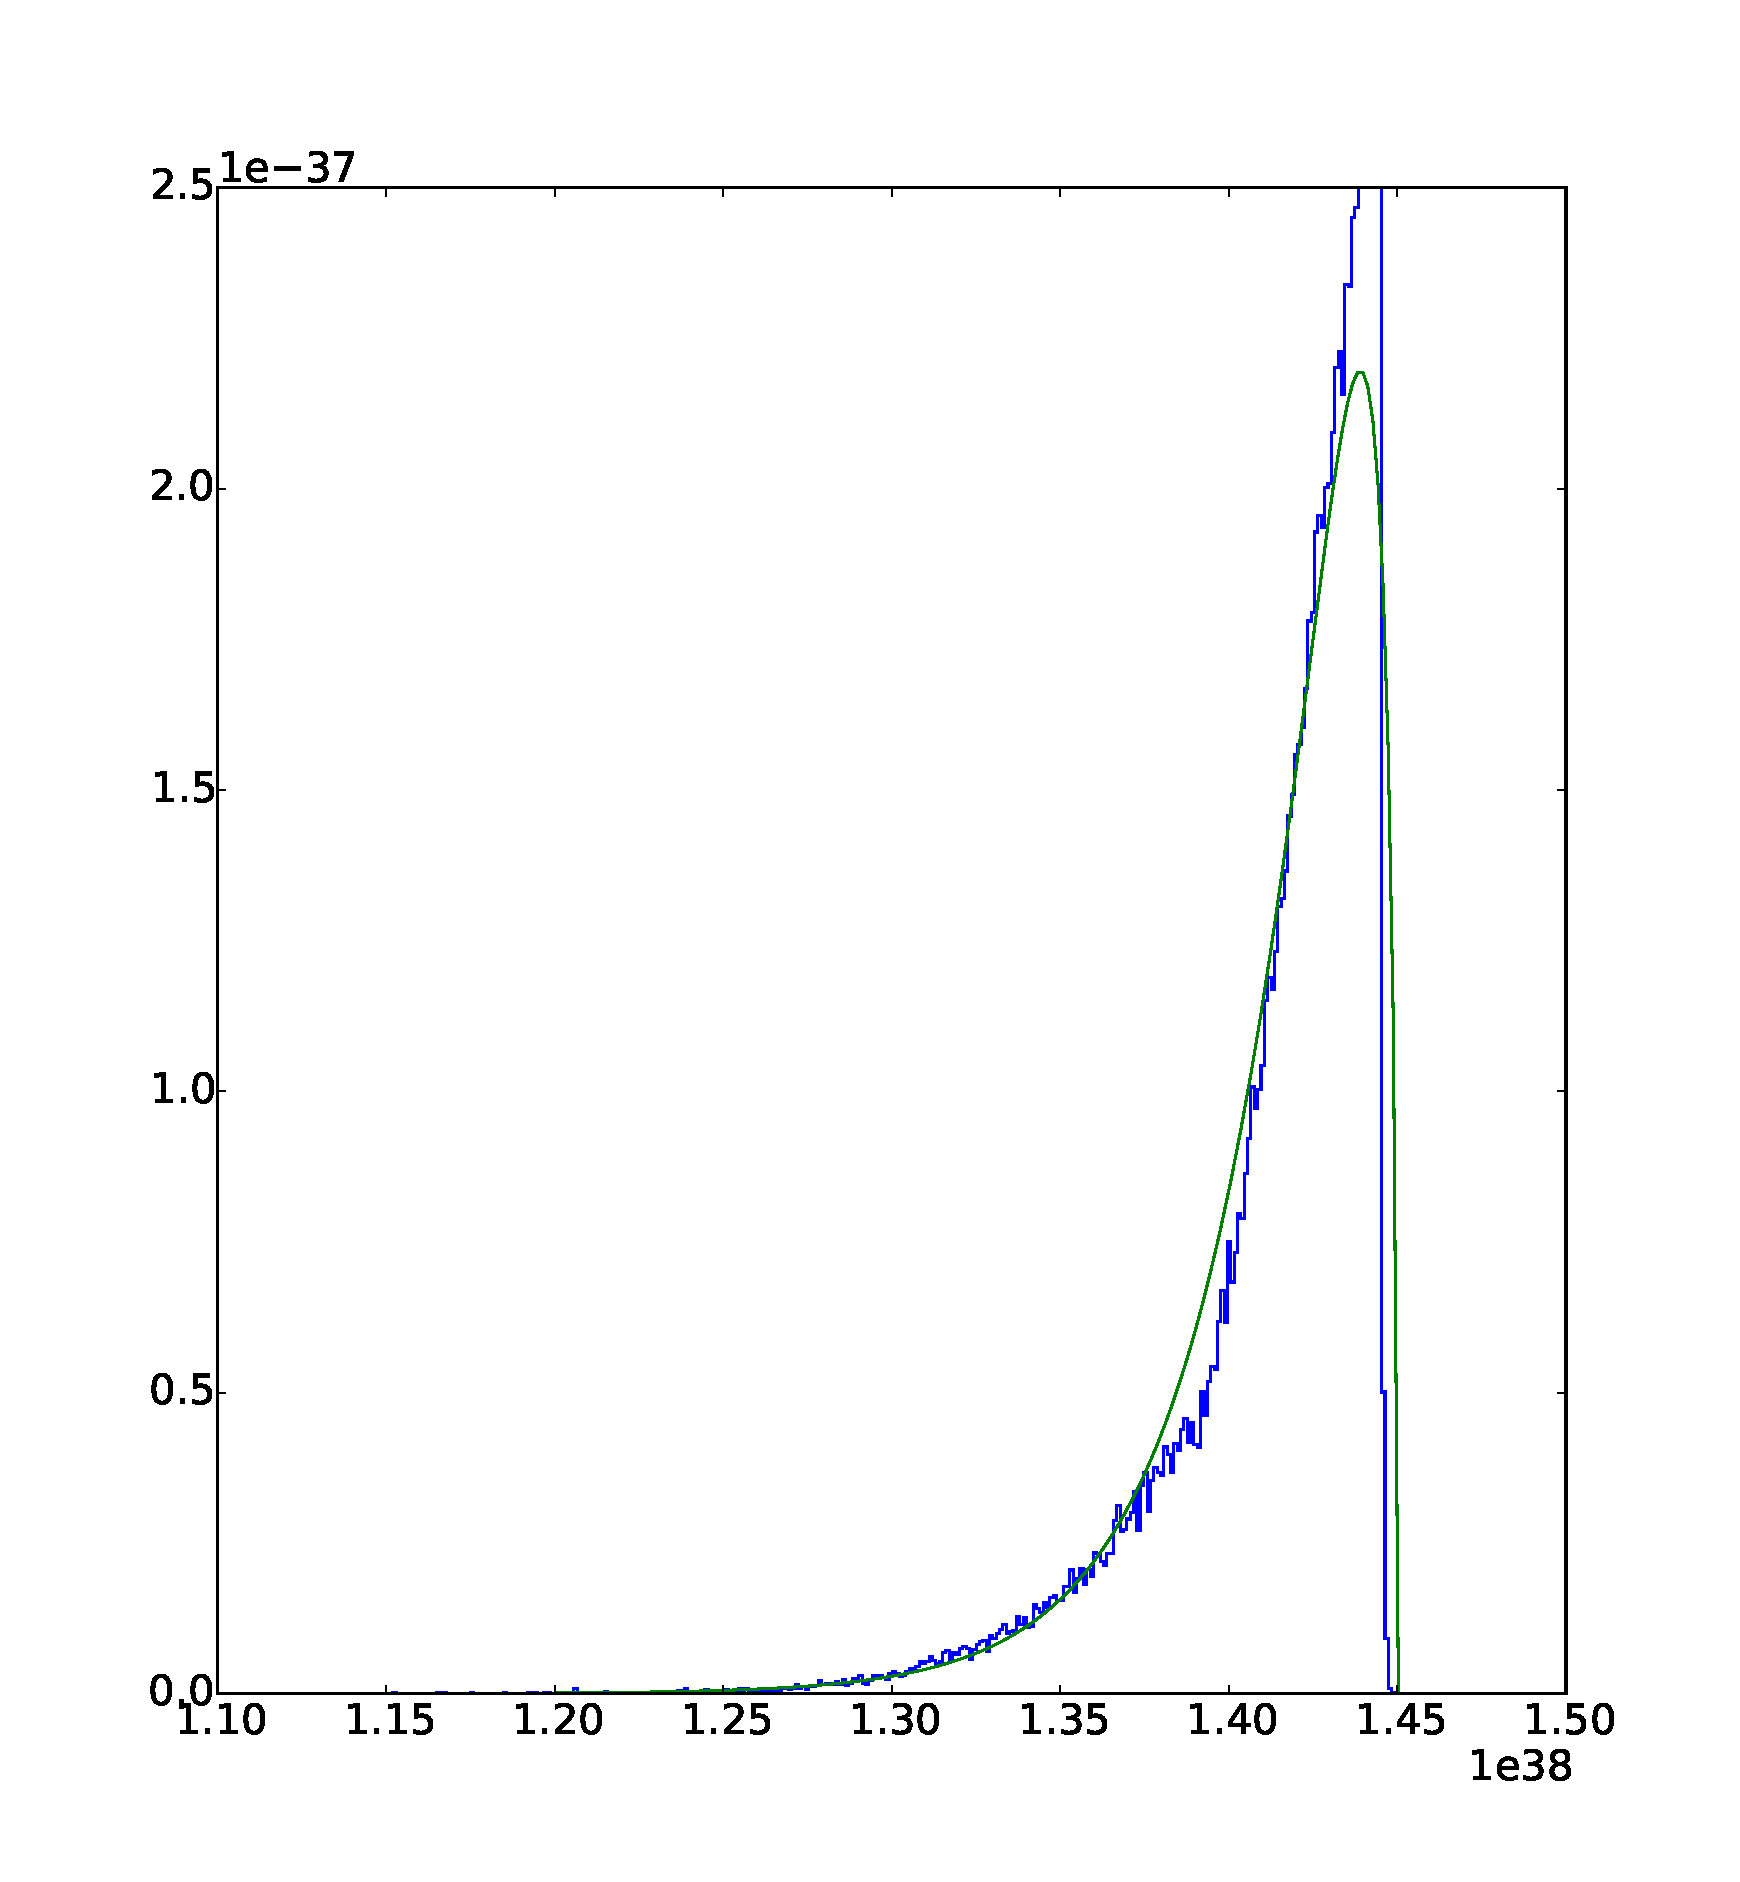
\includegraphics[width=\textwidth]{fit}
  \end{center}
  \caption{Distribution of luminosities of real packets.}
  \label{fig:hist}
\end{figure*}

For virtual packets, the luminosity distribution seems to depend
mildly on the frequency.  We do not know $P(\Lumi | 1, \vecth)$ before
we do the simulation and we do not know its functional form
either. But we want to minimize the assumptions on the form. Hence
seek a nonparametric description of the samples. Obviously, if we
observe $n_i=0$ or $n_i=1$, we cannot infer the distribution $P(\Lumi
| 1, \vecth)$ from such little information. If we may assume that
$P(\Lumi | 1, \vecth)$ varies only little with $i$, we may pool
together luminosities $l_{ij}, j=1 \dots n_i$, of adjacent bins to
form a handful of larger bins, say $10-100$, in which we assume the
distribution is constant and we have enough packets, at least $\sum_i
n_i \gtrsim 500$. The I propose we use Gaussian kernel density
estimation (KDE) to obtain a smooth estimate of $P(\Lumi | 1, \vecth)$
that we can evaluate at arbitray $\Lumi$. In python, the easiest way
to do this is via \texttt{scipy.stats.gaussian\_kde}. The fastest to
my knowledge is \texttt{figtree} but the difference will be mostly
irrelevant unless there $\sum_i n_i = 10^5$ packets in a combination
of bins.

Given the KDE estimate, we could compute the distribution for the sum
of two variables as the convolution
\begin{align}
  \label{eq:sum-of-2}
  P(\Lumi | N_i=2, \vecth) = \int \rmdx{l} P(\Lumi -l | N_i=1, \vecth) P(l | N_i=1, \vecth).
\end{align}
For $N_i =k$, we would repeat the procedure convolving $P(\cdot |
N_i=k-1, \vecth)$ and $P(\Lumi | N_i=1, \vecth)$ and each time we
would need a new KDE estimate and we would have to repeat the integral
for different values of $\Lumi$. This quickly gets out of hand and I
fear the errors due to KDE assumptions add up. In my attempts with
\texttt{mathematica}, the probability for many values of $\Lumi$ was
negative and the whole procedure is slow. Let's forget about it.

The more model-independent and faster approach is to use the
luminosity samples $\{l_j: j=1 \dots \sum n_i\}$ for all bins $i$ that
are combined. We can create samples of the sum of $N_i=2$ luminosities
by adding $l_1+l_2, l_3 + l_4 \dots$ and similarly for larger
$N_i$.

\subsubsection*{Approximation for large $n_i$}

For $N \gtrsim 15$, we can just use the central limit theorem
such that
\begin{align}
  \label{eq:clt}
  P(\Lumi | N_i, \vecth) \approx \gaussian \given{\Lumi}{N_i \times E[l], N_i \times V[l]}
\end{align}
and the expecation value and variance have to be estimated by the mean
and variance of the samples $\{l_j\}$. In fact, this paper~\cite{bohm_statistics_2014}
shows that the \emph{scaled Poisson} is a more accurate approximation
given the first and second moment. But the resulting integral can't be
solved exactly, so for easier calculation we stick with the Gaussian.

\subsubsection{Poisson noise}

Let us now consider $P(N_i | \vecth)$, the second term in
\eqref{eq:lum}. As stated before, we assume the number of packets in
the given simulation follows a Poisson distribution whose rate
parameter $\lambda_i = \lambda_i(\vecth)$ has to be inferred from the
observed $n_i = n_i(\vecth)$. We can use the law of total probability
\begin{equation}
  \label{eq:poisson-post-pred}
  P(N_i | \vecth) = \int \rmdx{\lambda_i} P(\lambda_i | \vecth) \poisson(N_i | \lambda_i, \vecth)
\end{equation}
and Bayes' theorem
\begin{equation}
  \label{eq:poisson-post}
  P(\lambda_i | \vecth) \propto \poisson(n_i | \lambda_i) P_0(\lambda_i)
\end{equation}
If we choose the noninformative and improper Jeffreys prior
$P_0(\lambda_i) \propto 1/\sqrt{\lambda_i}$ then we get the analytical
result~\cite[Eq. 5]{Aggarwal:2011aa}
\begin{align}
  \label{eq:post-pred-analytical}
  P\given{N_i}{\vecth} &= \frac{n_i! [2 (N_i + n_i)]!}{2^{N_i+n_i+1/2}4^{N_i} N_i! (2 n_i)! (N_i + n_i)!}\\
  &= \frac{(N_i + n_i + 1)_{N_i + n_i}}{(n_i + 1)_{n_i} \sqrt{2}\, 2^{3N_i + n_i}N_i!}
\end{align}
where
\begin{align}
  \label{eq:pochhammer}
  (a)_k \equiv a (a + 1) \dots (a + k - 1)
\end{align}
is the Pochhammer symbol.

In essence, $P(N_i | \vecth)$ is
the posterior predictive distribution to have $N_i$ packets given that
the simulation spit out $n_i(\vecth)$ packages. So $n_i$ is known,
while $N_i$ is a random variable and we take into account its
uncertainty by summing over $N_i$ in \refeq{lum}. This is relevant for bins where $n_i$ is small. If we got
2 packets, it is not so unlikely we could have gotten one package. But
of course with only half the packages, the expectation for the sum of
luminosities changes significantly.

\subsubsection*{Approximation for large $n_i$}

The mode and variance of $P(N_i | \vecth)$ are
\begin{align}
  \label{eq:poisson-mode-variance}
  \arg \max P(N_i | \vecth) = n_i -1, && V[N_i] = 2 n_i + 1.
\end{align}
Why is the variance $\sim 2 n_i$ and not $n_i$ as one would expect for Poisson? Variances are additive and we get one factor of $n_i$ from the Poisson in \refeq{poisson-post-pred} and another one from \refeq{poisson-post}.

For $n_i=0$, the distribution diverges at zero, a consequence of the
Jeffreys prior.  For $n_i \gtrsim 30$, the distribution can be well
approximated by a Gaussian
\begin{align}
  \label{eq:poisson-gauss-approx}
  P(N_i | \vecth) \approx \gaussian \given{N_i}{n_i-1, 2 n_i + 1}
\end{align}

\subsection{Putting it all together}

Now it is time to combine all the equations above to see what actually
needs to be implemented. The likelihood is
\begin{align}
  \label{eq:all-likelihood}
  P\given{\data}{\vecth} &= \prod_{i=1}^{N_b} \int \rmdx{\Lumi} P\given{\Lumi}{\vecth}   P\given{\data}{\Lumi}\\
  &= \prod_{i=0}^{N_b} \sum_{N_i=0}^\infty \int \rmdx{\Lumi} P \given{\Lumi}{N_i}
  P\given{N_i}{\vecth} P\given{\Lumi}{\mui, \sigi}
\end{align}


\subsubsection*{Large $n_i$}

If many packets are observed in bin $i$, then with good approximation
everything is Gaussian and we can evaluate the integral over $\Lumi$
analytically: the convolution of two Gaussians is another Gaussian
with variances added.

\begin{align}
  \label{eq:all-large-n}
P\given{\data}{\vecth}  &=  \prod_{i=1}^{N_b} \sum_{N_i=0}^\infty \int \rmdx{\Lumi} \gaussian \given{N_i}{n_i-1, 2 n_i + 1} \gaussian \given{\Lumi}{N_i  E[l], N_i V[l]}\\
  & \phantom{\prod_{i=1}^{N_b} \sum_{N_i=0}^\infty \int \rmdx{\Lumi}} \times \gaussian \given{\Lumi}{\mu_i, \sigma_i} \nonumber\\
  & = \prod_{i=1}^{N_b} \sum_{N_i=0}^\infty \gaussian \given{N_i}{n_i-1, 2 n_i + 1} \gaussian \given{N_i \El}{\mu_i, \sigi + N_i \Vl}
  % &= \frac{\left| \Vl \mui + \El \sigi \right|+ (\Vl \mui + \El \sigi) \erf\left(\frac{\sqrt{N_i} \left| \Vl \mui + \El \sigi \right|}{\sqrt{2 \sigi \Vl (\Vl N_i + \sigi)}}\right)}{}\\
%   &= \frac{1 + \sgn(\rho) \erf\left(\frac{\sqrt{N_i} \left| \rho \right|}{\sqrt{2 \sigi \Vl \xi}}\right)}{4 \pi \sqrt{(2n_i + 1) \xi}} \exp \left(-\frac{ (N_i \El -\mui)^2}{2  \xi}\right)
% \\
%   &\phantom{=} \times \exp \left(\frac{(2n_i+1) (N_i \El)^2 + N_i^3 \Vl - 2(2n_i+1)N_i \El \mui + (2n_i+1) \mu^2}{2 (2n_i + 1) \xi}\right) \nonumber\\
%   &\phantom{=} \times \exp \left(\frac{(n_i-1)^2 \sigi + (n_i - 1) N_i ((n_i-1)\Vl - 2\sigi) + N_i^2 (-2(n-1)\Vl + \sigi)}{2 (2n_i + 1) \xi}\right) \nonumber
\end{align}
% where
% \begin{align}
%   \label{eq:rho}
%   \rho &\equiv  \Vl \mui + \El \sigi\\
%   \xi &\equiv N_i \Vl  + \sigi
% \end{align}

For each bin, we have to compute a series. We have three options:
\begin{enumerate}
  \item The quick and dirty approach is to approximate $\sum_{N_i}$ by
  $\int \rmdx{N_i}$ and use \texttt{scipy.integrate.quad} to
  numerically integrate.
  \item If the first approach turns out to be too slow, we can just
  sum up a finite number of terms as the summand quickly falls off for
  large $N_i$; cf. \reffig{series}. The summand/integrand is unimodal
  and well behaved. For the numbers I tried, the mode was near $n_i$
  as implied by the first Gaussian. The mode can be computed
  analytically but the expression is very long, so I don't show it
  here. We could start summing from there and grow to the left and
  right until terms become negligibly small. In my tests in
  mathematica, I chose the number of terms by eye.
  \item The third and fastest way would be to compute the mode, then
  use the Laplace approximation to estimate the integral. This
  requires the 2nd derivative around the mode, which is available in
  closed form but too long to report here. Check the mathematica
  notebook for the explicit results.
\end{enumerate}
For tests I did, the first two agreed within 5 or 6 digits, and the
Laplace approximation good to the 3rd digit, so we might want to go
with that, as it should be the fastest.

For $N_i \to 0$, the summand is independent of $\El$ and $\Vl$ and
very small if $n_i$ is large, so there is fortunately no special case
to take care of.

\begin{figure}[h]
  \centering
  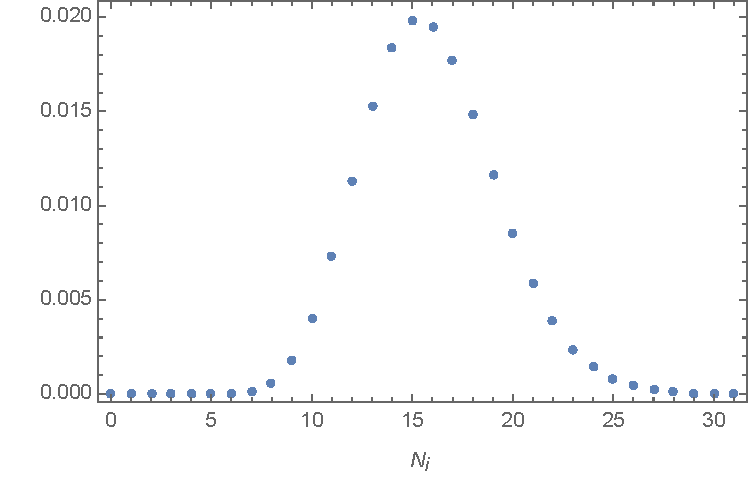
\includegraphics{series}
  \caption{Series summand $\gaussian \given{N_i}{n_i-1, 2 n_i + 1}
    \gaussian \given{N_i \El}{\mu_i, \sigi + N_i \Vl}$ of
    \refeq{all-large-n} for various values of $N_i$ and $\mui=5,
    \sigi=5^2,n_i=15, \El= 0.9 * \mui / n_i, \Vl=0.1$.}
  \label{fig:series}
\end{figure}

\subsubsection*{General case}

Plugging in the KDE estimates of $P\given{\Lumi}{N_i}$, we cannot use
the Laplace approximation because the mode and the derivative there
are not known. For small $n_i$, typically few terms in the series
contribute, so the number of numerical integrals can be kept
small. However, this depends on the experimental uncertainty. If it is
large, then we have to take into account more terms.

It is worth noting that for $N_i=0$, $\Lumi$ would be the sum of zero
terms and that is ill defined. So we have to start summing at
$N_i=1$. But that does not mean that $n_i=0$ is invalid, too. In fact,
$P(N_i=1 | n_i=0) = 17.7\%$ in our model with the Jeffreys prior. So
no packets seen means you could have seen a packet with some sizable
probability. Of course this is a simplification. Looking at a spectrum
in which the last 1000 bins didn't get a packet and the luminosity
drops before that, I associate a much smaller probability for $N_i=1$
in the very last bin than in bin $N_b-1000$. The difference is because
I take into account extra information: smoothness of the spectrum,
monotonicity \dots. At present, I don't know how to encode this in the
model \emph{and} keep it computationally tractable. It is left as an
exercise for the reader.

\subsubsection*{Recommendation}

The strategy would be to look at each bin separately. If $n_i \gtrsim
5$, use the large-$n_i$ approach from above. Else start at $N_i=1$ and
sum the numerical integrals until it is $10^{-4}$ of the maximum
term. For 10000 bins, this works can be parallelized easily.

For the real packets, I compared the general approach to the Gaussian
large-$n_i$ approximation, using numerical integration in both cases
in \texttt{mathematica}. For $n_i=1\dots5$, the difference is slighly
less than 10\%. From $n_i=10$ to 15, it drops from 5\% to 3\% level,
and for $n_i=100$, both approaches agree to within $10^{-4}$. Laplace
can be used from $n_i=5$ on. In all cases except $n_i=100$, the
Gaussian approximation is systematically \emph{below} the general
result.

If we are ok with less than 10\% error, we can employ the Gaussian
approximation from $n_i\ge5$, which means we neglect the 3rd and
higher moments of the luminosity distribution. If the virtual packets
are even more skewed than the real packets, we might need to start at
$n_i \sim 10$.

\section{Priors}

\subsection{Polychord}

The polychord program only performs sampling and integration on the
unit hypercube with coordinates $\vecu$. Furthermore, it assumes that
the prior in these coordinates is uniform
\begin{equation}
  \label{eq:hypercube-prior}
  P(\vecu) = 1.
\end{equation}
In each iteration, we have to return the log likelihood for given
$\vecu$ passed in by polychord.  As above, suppose $\vecth$ represents
the parameters that are fed into the tardis simulation, then we need
to find the transform $\vecth(\vecu)$. The prior transforms as
\begin{equation}
  \label{eq:par-trafo}
  P(\vecth) \rmdx{\vecth} =  P(\vecu) \rmdx{\vecu},
\end{equation}
so with the flat prior
\begin{equation}
  \label{eq:par-trafo-likelihood}
  P(\vecth) = \left| \frac{\partial \theta_i}{\partial u_j} \right|^{-1} .
\end{equation}
There are two options:
\begin{enumerate}
\item \label{direct-transform} We can find $\vecth(\vecu)$ such that
  the Jacobian on the right in \refeq{par-trafo-likelihood} is the
  prior we want. The we just compute $\log L(\vecth(\vecu))$ for every
  sample $\vecu$ polychord provides.
\item If \ref{direct-transform} is not possible, we need to divide
  out the Jacobian and multiply by the actual prior we want, so for
  polychord we pretend we have a uniform prior and an \emph{effective} likelihood
  \begin{equation}
    \label{eq:eff-likelihood}
    L'(\vecu) = L(\vecth(\vecu)) P(\vecth(\vecu)) \left| \frac{\partial \theta_i}{\partial u_j} \right|
  \end{equation}
\end{enumerate}
Nested sampling is most efficient if the prior is close to the
posterior as measured by the relative entropy or Kullback-Leibler
divergence~\cite{skilling_nested_2006}. We therefore prefer
option~\ref{direct-transform}. While it restricts us to simple forms
of priors: uniform, Gaussian, or Dirichlet, this, fortunately, is
enough for our purposes. The explicit transformation is given below,
separately for each block of parameters.

% We could try to work out the
% transformation $\vecth(\vecu)$ such that the transformed prior has the
% form we want but for the relative abundances I don't know how to do
% that. Hence we will keep it simple and pretend that our prior is
% uniform and move everything into the effective likelihood $L'$. This
% amounts to perhaps slightly less efficient sampling but more
% importantly we can correctly define the target density from samples
% are produced. The Jacobian determinant can be computed as the product
% over blocks of correlated parameters.

\subsection{Relative abundances}

\subsubsection{Transformation}

Suppose we have $K$ abundances subject to the constraints
\begin{align}
  \label{eq:unit-simplex}
  & 0 \leq \theta_k \leq 1, & \sum_{k}\theta_k = 1.
\end{align}
In other words, the abundances are defined on the unit simplex.  As
shown in~\cite{betancourt_cruising_2012}, we can directly transform
$\vecu$ with $\dim \vecu = K$ to $\vecth$ as follows. First create $K$
Gamma variates with the inverse-transform method, in python code
$\xi_k = \texttt{scipy.stats.gamma.ppf}(u_k, \alpha_k)$ with the shape
parameter $\alpha_k$ explained below. Then normalize the samples as
\begin{equation}
  \label{eq:dirichlet-gamma}
  \theta_k = \frac{\xi_k}{\sum_{k'} \xi_{k'}}.
\end{equation}
such that
\begin{equation}
  \label{eq:dirichlet-prior}
  P(\vecth) = \Dirichlet(\vecth | \alpha)
\end{equation}

\subsubsection{Prior information}

The canonical choice of a prior for fractions such as relative
abundances is the Dirichlet
distribution~\cite[App.~B]{bishop_pattern_2006}
\begin{equation}
  \label{eq:dirichlet-def}
  \Dirichlet \given{\vecth}{\vecalpha} = \frac{\Gamma\left(\sum_k \alpha_k\right)}{\prod_k \Gamma(\alpha_k)} \prod_{k=1}^K \theta_k^{\alpha_k-1}
\end{equation}
and depends on $K$ parameters $\vecalpha$. How to choose $\alpha_k$?
The mode of $\theta_k$ is $\frac{\alpha_k - 1}{\sum_k (\alpha_k -
  1)}$, so we should choose $\alpha_k > 1$ if we want a well defined
mode. For prior ignorance, we want $\alpha_k$ identical. The canonical
choice of an uninformative distribution is a uniform distribution on
the unit simplex given by $\alpha_k=1 \, \forall \,
k$~\cite{tuyl_posterior_2009}.

Now suppose we want to include the available prior information. The
actual numbers come from table 5.1 of Wolfgang's thesis. He lists
constraints of the type
\begin{equation}
  \begin{aligned}[t]
    \label{eq:abundance-constraints}
    \mbox{C}  &< 12.5 \%,\\
    \mbox{Si} &>1 \%,\\
    1 &<\mbox{Si/S ratio} < 10 .
  \end{aligned}
\end{equation}
The most straightforward approach is to incorporate them as hard cuts
into the prior, leading to a new normalization. We will have to refine
this strategy if the regions of high posterior probability turn out to
be very close to the cuts. Formally, suppose $V$ is the subvolume of
the unit simplex in which all constraints are satistfied. Outside of
$V$, we set $P(\vecth) \equiv 0$. In the code, a sequence of
\texttt{if} statements incorporates the constraints. If any is
violated, the prior on the log scale is $-\infty$ and no tardis
simulation needs to be run. Our prior thus becomes
\begin{equation}
  \label{eq:abundances-prior}
  P(\vecth) = C_V^{-1} \mathbf{1}_V(\vecth) \Dirichlet\left(\vecmu(\vecth) \middle| \vecalpha=(10^{-4}, \dots, 10^{-4})\right) \boldsymbol{\theta}
\end{equation}
where the normalization constant $C_V$ is  determined from
\begin{equation}
  \begin{aligned}
    \label{eq:abundance-normalization}
    1 &= \int \rmdx{\vecth} P(\vecth)\\
    \Rightarrow C_V  &= \int_V \rmdx{\vecth} \Dirichlet\left(\vecmu(\vecth) \middle| \vecalpha=(10^{-4}, \dots, 10^{-4})\right)
  \end{aligned}
\end{equation}
and $\mathbf{1}_V$ is the indicator function on $V$; i.e.,
$\mathbf{1}_V(\vecth) = 1$ iff $\vecth \in V$.  If we keep the cuts
fixed, we only need to determine $C_V$ once. We can do that with good
precision without nested sampling by using the law of large numbers as
\begin{equation}
  \label{eq:abundances-large-numbers}
  C_V \approx \frac{1}{N} \sum_{i=1}^N \mathbf{1}_V(\vecth), \; \vecth \sim \Dirichlet\left(\vecmu(\vecth) \middle| \vecalpha=(10^{-4}, \dots, 10^{-4})\right)
\end{equation}
and drawing directly from $\Dirichlet(\vecalpha)$ using
\texttt{scipy.random.dirichlet}. However, we don't really need to
normalize our densities properly unless we compare different
models. In the near future, we will only infer the parameters of a
single model so there is no need to compute $C_V$.

\subsection{Other parameters}

For all parameters other than abundances we choose uniform priors to
start with. This is not necessarily noninformative but we should be a
proxy for a diffuse prior hoping that the likelihood is sharp enough
to constrain all parameters. In the end, we should study the prior
dependence by choosing some other distribution such as wide Gaussians
or Cauchys to see if it has a significant effect.

\bibliography{references}

\end{document}
